% Created 2024-12-17 Tue 00:14
% Intended LaTeX compiler: pdflatex
\documentclass[11pt]{article}
\input{../../../preamble.tex}
% setting up title page
\title{
  
\includegraphics[width=0.4\textwidth]{fmf_logo}\\
  {\small Oddelek za fiziko} \\
  {Osnove mikrovalovne tehnike}\\
  {\small Poročilo pri FP5}\\

}
\date{}
\author{ Kristofer Č. Povšič, 28211104 \\[5 cm]
 \small  Asistent: Tilen Knaflič \\
}

\addbibresource{refs.bib}
\begin{document}

\maketitle
\tableofcontents

\section{Uvod}\label{sec:orge7c61fa}

Energije žarkov ne merimo neposredno, ampak le posredno tako, da izmerimo energijo elektronov, ki jo le ti prejmejo od žarkov \(\gamma\) pri fotoefektu, Comptonovem sipanju ali pa energijo parov pozitron-elektron iz procesa tvorbe parov. Scintilator
je material, ki je scintilabilen. To pomeni, da zažari, ko je vzburjen zaradi
radioaktivnega sevanja. Pri scintilacijskem detektorju uporabljamo v ta namen monokristale natrijevega jodida (NaI) z dodatkom okrog \(1 \%\) talija (Tl) kot nečistoče.

Pri potovanju hitrih nabitih delcev skozi kristal ostane za njimi razdejanje v obliki sledi elektron-vrzel. Ponovno združevanje med elektroni in vrzelmi poteka energijsko ugodneje v bližini atoma nečistoče. Vrzeli vzamejo elektronom atomom Talija in jih ionizirajo. Elektroni se nato rekombinirajo s temi ioniziranimi atomi nečistoč. Odvečna energija gre bodisi sosednjim atomom v kristalni mreži, kar poveča termično gibanje ali pa z izsevanjem fotonov vidne svetlobe.

Število scintilacijskih fotonov določimo s pomočjo fotopomnoževalke. Višina signala iz fotopomnoževalke, ki signal ojača, je sorazmerna številu fotonov in torej tudi energiji, ki jo hitri nabiti delec izgubi v scintilatorju.

Sunek iz fotopomnoževalke pošljemo skozi predojačevalnik, ojačevalnik ter mu izmerimo napetostno višino z amplitudnim analizatorjem.
\subsection{Fotoefekt}\label{sec:orgf12cecc}

Pri fotoefektu žarek \(\gamma\) izbije elektron iz enega od vezanih stanj. Najverjetneje je to elektron iz lupine K. Atom, ki je po emisiji elektrona K v vzbujenem stanju, se vrne v osnovno stanje tako, da zapolni vrzel z elektronom iz višjih, manj vezanih stanj.
Pri tem izseva karakteristični žarek X. Tudi ta v scintilatorju lahko doživi
fotoefekt na manj vezanih elektronih in dobimo dva elektrona, katerih
energija je približno enaka prvotnemu fotonu \(\gamma\). Nekateri
karakteristični žarki pa uidejo iz
scintilatorja in s tem dobimo vrh pobega fotona pri \(E = E_{\gamma} - E_K\),
kjer je \(E_K\) vezavna energija elektrona.
\subsection{Comptonovo sipanje}\label{sec:org322b661}

Comptonovo sipanje je neelastično sipanje fotona na skoraj prostem elektronu.
Pri sipanju se seveda ohranjata energija in gibalna količina. Spekter
comptonsko sipanih elektronov je zvezen. Elektroni se sipajo pretežno naprej,
fotoni pretežno nazaj. Izrazit rob t.i. Compton edge, izgine, saj se
nekateri od nazaj sipanih žarkov \(\gamma\) absorbirajo v scintilatorju in
so vidni v fotovrhu (oz. vrh popolne absorbcije).
Pri \(E_{\gamma min}\) se pojavi majhen vrh (vrh povratnega sipanja, ang.
\emph{back-scattering peak}). Ta pripada fotonom, ki so se sipali nazaj v steklu,
ki prekriva oscilator ali pa v steklu fotopomnoževalke in se nato absorbirali
v scintilatorju.
\subsection{Tvorba parov}\label{sec:org4af1b3a}

Kadar ima žarek \(\gamma\) dovolj energije (\(E_{\gamma} \ge 1.02 \mathrm{MeV}\)),
se lahko v bližini jedra spremni v par pozitron-elektron s skupno kinetično
energijo \(E_{\gamma} - 2 m_0 c ^2\), odvečno gibalno količino pa prevzame
jedro. Nastala delca se gibljeta pretežno v smeri naprej. V scintilatorju se
zaustavita in mu predata svojo kinetično energijo. Ob upočasnitvi se pozitron
z enim od elektronov, ki jih sreča na svoji poti, anihilira. Nastaneta dva
kolinearna žarka \(\gamma\). Možno je, da pobegneta oba, samo en ali pa oba
ostaneta v scintilatorju. Tako dobimo vrh dvojnega pobega, vrh pobega in vrh
polne absorpcije.
\section{Potrebščine}\label{sec:orgaba5d65}
\begin{itemize}
\item scintilacijski detektor
\item izvor visoke napetosti za napajanje fotopomnoževalke
\item ojačevalnik z enokanalnim analizatorjem
\item večkanalni analizator
\item radioaktivni izvor \(^{22} \mathrm{Na}, \ ^{137} \mathrm{Cs} \text{ in } ^{60} \mathrm{Co}\)
\end{itemize}

\section{Naloge}\label{sec:org6346c70}
\begin{enumerate}
\item Ojačene signale iz scintilacijskega detektorja si poglej osciloskopu. K poročilu priloži zaslon ali pa skico signalov.
\item Z enokanalnim analizatorjem izmeri spekter natrija in nariši graf.
\item S pomočjo dveh črt \(\gamma\) iz natrija z energijo \(E_1 = 0.51 \mathrm{MeV}\)
in \(E_2 = 1.277 \mathrm{MeV}\) umeri energijsko skalo scintilacijskega
spektrometra (večkanalni analizator) in izmeri energijo Črt \(\gamma\) iz
cezija in kobalta. Pri analizi od izmerjenega spektra odštej spekter ozadja.
\item Izmeri energijsko ločljivost za vrh popolne absorpcije tako, da podatkom v
okolici vrha prilagajaš Gaussovo funkcijo. Izmeri ločljivost za vrhove pri
različnih energijah - uporabi meritve spektrov natrija, cezija in kobalta.
\item Izračunaj izkoristek kristala za vrh popolne absorpcije (določi z izvorom
\(^{137} \mathrm{Cs}\))
\item Oceni energijo vrha povratnega sipanja
\end{enumerate}
\section{Izračuni in obdelava}\label{sec:org8f92a5e}
Za obdelavo podatkov sem uporabil Python in njegove knjižnice numpy, matplotlib, cmasher, scipy, uncertainties ter pandas. Poleg tega sem uporabljal tudi AMPTEK Display and Acquisition Software.

\subsection{Enokanalne meritve}\label{sec:orgb677120}

Podatke sem za vsak interval energije zbiral desetkrat po \(10 \mathrm{s}\), kar sem potem izpovprečil in dobil tudi standardno deviacijo, kakor lahko vidimo na \ref{fig:eno}.

Globalen interval energije je bil 8 enot na merilni napravi, okno (ang. window) na napravi pa je bilo 0.4, zato da sem pomeril 20 meritev.

\begin{slika}[H]
\begin{center}
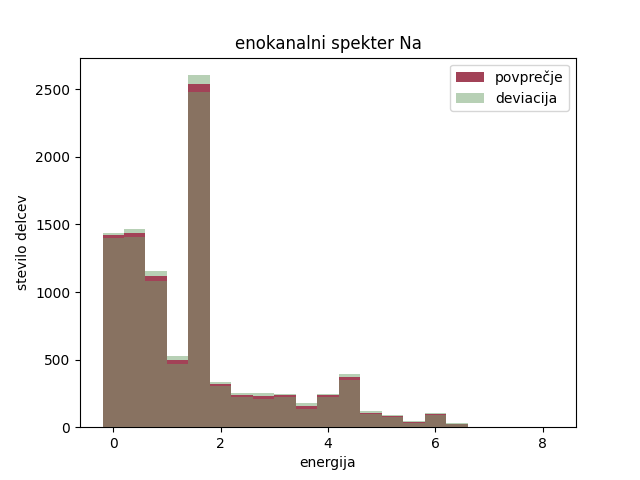
\includegraphics[width=.9\linewidth]{figures/enokanalni_na.png}
\caption{\small Graf prikazuje enokanalne meritve $^{22} \mathrm{Na}$. Meritev je bila opravljena desetkrat po $10 \mathrm{s}$, kar sem potem izpovprečil ter izračunal tudi standardno deviacijo. } \label{fig:eno}
\end{center}
\end{slika}

\subsection{Umeritev energijske skale}\label{sec:orgb47b656}

Energijsko skalo sem umeril s pomočjo znanih vrhov energij natrija, ki sta bila napisana v navodilih.

\begin{slika}[H]
\begin{center}
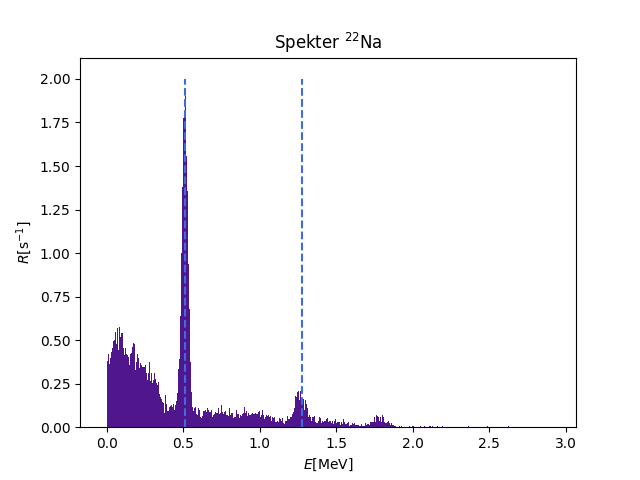
\includegraphics[width=.9\linewidth]{figures/kalibracija.png}
\caption{\small Graf kalibracije meritev. Kalibrirali smo s pomočjo znanih vrhov natrija. }
\end{center}
\end{slika}

\subsection{Šum ozadja}\label{sec:org39e42a5}

Podatke za šum ozadja sem zbiral 11 minut in tako dobil graf \ref{fig:sum}

\begin{slika}[H]
\begin{center}
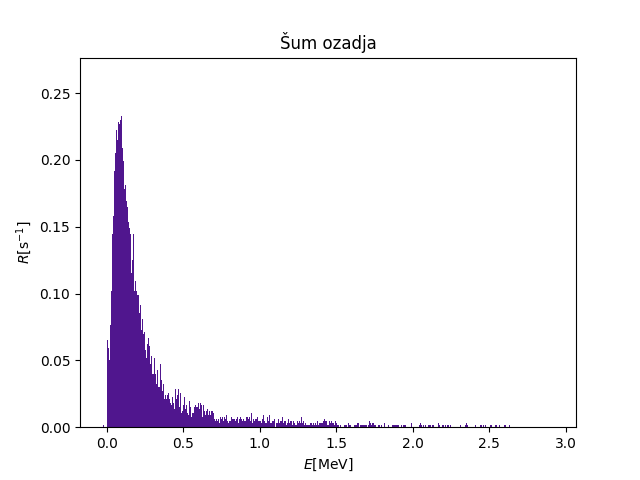
\includegraphics[width=.9\linewidth]{figures/ozadje.png}
\caption{\small Graf prikazuje šum ozadja, ki se ga je merilo 11 minut. }\label{fig:sum}
\end{center}
\end{slika}

\subsection{Spekter \(^{22} \mathrm{Na}\)}\label{sec:org0586687}

Z umerjeno energijsko skalo sem sedaj narisal skalibriran spekter natrija z regresiranimi krivuljami za oba energijska vrhova.

\begin{slika}[H]
\begin{center}
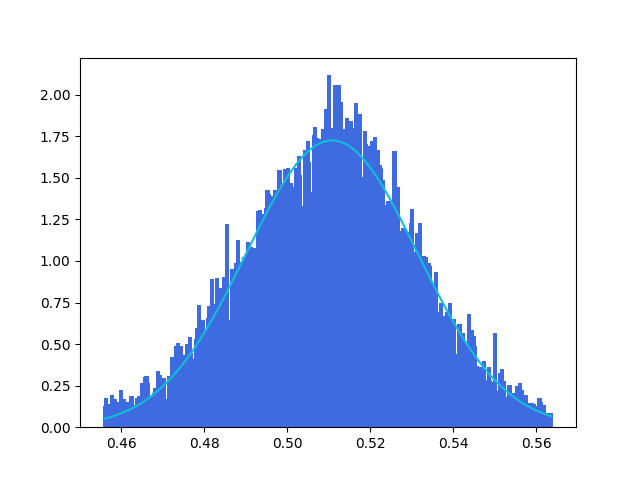
\includegraphics[width=.9\linewidth]{figures/na22_no_bg.png}
\caption{\small Graf spektra $^{22} \mathrm{Na}$ z regresiranimi Gaussovimi funkcijami na energijskih vrhovih}
\end{center}
\end{slika}

S pomočjo \ref{eq:1} sem izračunal pri vseh spektrih, kje naj bi bila energija Comptonovega roba

\begin{equation}
\label{eq:1}
E_{Compt} = \frac{E_{\gamma}}{1 + 2 \frac{E_{\gamma}}{m_0 c ^2}} \cdot 2 \frac{E_{\gamma}}{m_0 c ^2}
\end{equation}

Z enačbo \ref{eq:2} sem izračunal pri vseh spektrih tudi energijo povratnega sipanja

\begin{equation}
\label{eq:2}
E_{min} = \frac{E_{\gamma}}{1 + 2 \cdot \frac{E_{\gamma}}{m_0 c ^2}}
\end{equation}

kjer je \(m_0 c ^2 = 0.511 \mathrm{MeV}\) mirovna energija elektrona.

Za natrij dobim vrednosti:

\begin{align*}
E_{Compt} &= (0.34 \pm 0.01) \mathrm{MeV} \\
E_{min} &= (0.17 \pm 0.01) \mathrm{MeV}
\end{align*}

\subsection{Spekter \(^{60} \mathrm{Co}\)}\label{sec:org51e535e}

S prej umerjeno energijsko skalo sem sedaj lahko narisal in tudi dobil vrednosti energijskih vrhov kobalta. Energiji, ki sem jih dobil, sta

\begin{align*}
  E_1 &= (1.16 \pm 0.01) \mathrm{MeV} \\
E_2 &= (1.33 \pm 0.01) \mathrm{MeV}
\end{align*}

Po viru \autocite{noauthor_cobalt-60_nodate} naj bi bila energijska vrhova pri vrednostih \(E_{1vir} = 1.173 \mathrm{MeV}\) in \(E_{2vir} = 1.332 \mathrm{MeV}\), kar se znotraj napake ujema z danima rezultatoma.

\begin{slika}[H]
\begin{center}
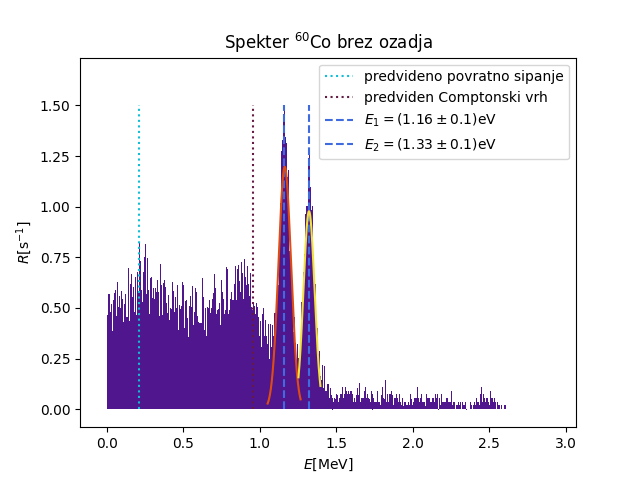
\includegraphics[width=.9\linewidth]{figures/Co60_no_bg.png}
\caption{\small Graf spektra $^{60} \mathrm{Co}$ z regresiranimi Gaussovimi funkcijami na energijskih vrhovih. }
\end{center}
\end{slika}

Za kobalt sem dobil sledeče vrednosti energije Comptonovega roba in povratnega sipanja
\begin{align*}
  E_{Compt} &= (0.95 \pm 0.01) \mathrm{MeV} \\
E_{min} &= (0.20 \pm 0.01) \mathrm{MeV}
\end{align*}
\subsection{Spekter \(^{137} \mathrm{Cs}\)}\label{sec:org8835c43}

Podobno kot za kobalt, sem tudi za cezij dobil energijo

\[ E_1 = (0.66 \pm 0.01) \mathrm{MeV}
\]

Prav tako je v okviru napake v redu z virom \autocite{noauthor_rich_2020}, katere vrednost je \(E_{1vir} = 0.66 \mathrm{MeV}\)

\begin{slika}[H]
\begin{center}
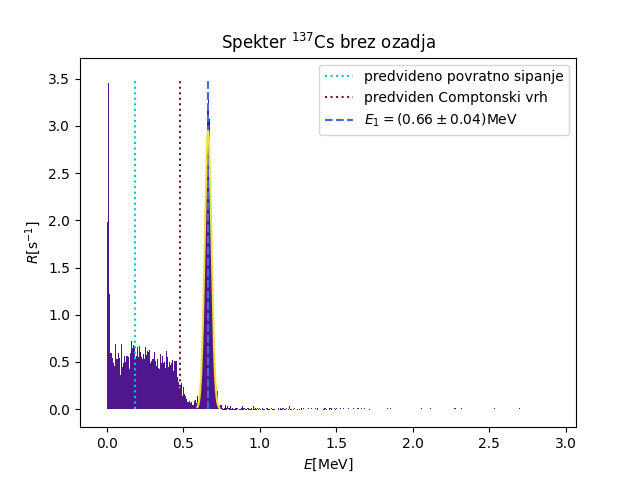
\includegraphics[width=.9\linewidth]{figures/Cs137_no_bg.png}
\caption{\small Graf spektra $^{137} \mathrm{Cs}$ z regresirano Gaussovo krivuljo na energijskem vrhu. }
\end{center}
\end{slika}

Za cezij sem dobil sledeče vrednosti

\begin{align*}
  E_{Compt} &= (0.47 \pm 0.01) \mathrm{MeV} \\
E_{min} &= (0.18 \pm 0.01) \mathrm{MeV}
\end{align*}
\subsection{Energijska ločljivost}\label{sec:orgfb9b95f}

Energijska ločljivost se spreminja z energijo in sicer narašča z energijo zaradi lastnosti napake pri Poissonovih procesih. Dobil sem

\begin{align*}
  R_{Na1} &= 0.095 \pm 0.001 \\
R_{Na2} &= 0.067 \pm 0.001 \\
R_{Co1} &= 0.083 \pm 0.001 \\
R_{Co2} &= 0.064 \pm 0.001 \\
R_{Cs} &= 0.078 \pm 0.001
\end{align*}
\subsection{Ocena izkoristka}\label{sec:orgb8fc457}

Za vzorec cezija imamo podan začetno aktivnost \(A_0 = 9250 s^{-1}\) leta 2013. Aktivnost pada s časom kot

\[ A(t) = A_0 e^{- \frac{t}{\tau}}
\]

Po 11 letih naj bi bila aktivnost \(A = 6416 \pm 100 s ^{-1}\). Izkoristek, ki je potem kvocient rezultata in pomerjene aktivnosti je potem

\[ \eta = (0.034 \pm 0.001)
\]
\section{Komentar}\label{sec:orgacaf9d4}

Vaja je bila uspešna. Grafi in energijske vrednosti vrhov se ujemajo z literaturo in tudi energijska ločljivost je smiselna. Edina stvar, ki ni smiselna je nizka ocena izkorista, saj je pri pičlih \(3 \%\). Smiselno bi bilo meritev ponoviti in ponovno opraviti izračun koeficient. Možno pa je tudi, da je pri izračunih prišlo do napake, vendar je jaz nisem našel.

\printbibliography[heading=bibintoc]
\end{document}
